\PassOptionsToPackage{table}{xcolor}
\documentclass[pdf]{beamer}
\mode<presentation>{\usetheme{Dresden}}
\usepackage{lmodern}
\usepackage[normalem]{ulem}
\usepackage{amsmath,textcomp,amssymb,geometry,graphicx,listings,array,color,amsthm}
\usepackage{multirow}

\usepackage[noend]{algpseudocode}

\usepackage[
backend=biber,
sorting=ynt,
]{biblatex}
\addbibresource{lecture.bib}

\usepackage{tikz}
\usepackage{multicol}
\usetikzlibrary{shapes,snakes}
\usetikzlibrary{positioning}
\usetikzlibrary{arrows}
\usetikzlibrary{fit}
\usetikzlibrary{math}

%% For on-slide alerting of nodes
\tikzstyle{alert} = [text=black, fill=blue!20, draw=black]
\setbeamercolor{alerted text}{fg=blue}
\tikzset{alerton/.code args={<#1>}{%
  \only<#1>{\pgfkeysalso{alert}} % \pgfkeysalso doesn't change the path
}}

%% utils for removing uninteresting sections from the navbar
%% https://tex.stackexchange.com/questions/317774/hide-section-from-sidebar
\makeatletter
\let\beamer@writeslidentry@miniframeson=\beamer@writeslidentry%
\def\beamer@writeslidentry@miniframesoff{%
  \expandafter\beamer@ifempty\expandafter{\beamer@framestartpage}{}% does not happen normally
  {%else
    % removed \addtocontents commands
    \clearpage\beamer@notesactions%
  }
}
\newcommand*{\miniframeson}{\let\beamer@writeslidentry=\beamer@writeslidentry@miniframeson}
\newcommand*{\miniframesoff}{\let\beamer@writeslidentry=\beamer@writeslidentry@miniframesoff}
\makeatother

%% preamble
\title{TLE Differencing}
\subtitle{Post Hoc Uncertainty Estimation}
\author{A.C.}
\date{\today}

\AtBeginSection[]
{
  \miniframesoff
  \begin{frame}{Outline}
    \tableofcontents[currentsection,hideothersubsections]
  \end{frame}
  \miniframeson
}

\definecolor{darkred}{rgb}{0.7,0,0}
\definecolor{darkgreen}{rgb}{0,0.5,0}
\definecolor{darkblue}{rgb}{0,0,0.5}
\definecolor{darkpurple}{rgb}{0.4, 0.0, 0.4}

%% Code font settings
\lstset{
  showstringspaces=false,
  basicstyle=\scriptsize\ttfamily,
  commentstyle=\color{darkred},
  stringstyle=\color{darkgreen},
  keywordstyle=\bfseries\color{darkpurple},
}

%%%%%%%%%%%%%%%%%%%%%%%%%%
% Start of Actual slides %
%%%%%%%%%%%%%%%%%%%%%%%%%%
\begin{document}
\begin{frame}
  \titlepage
\end{frame}

\section{TLE Primer}
\subsection{Kepler Theory}
\begin{frame}{Conic Perfection}
  \only<1>{
    \[ \ddot{r} = \frac{\mu}{r^2} \]
  }
  \only<2>{
  \begin{center}
    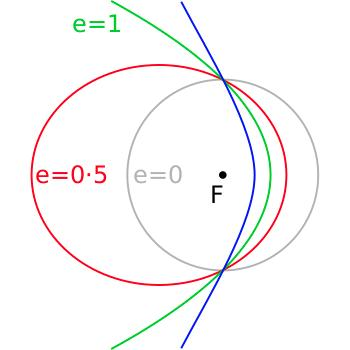
\includegraphics[scale=0.4]{images/OrbitalEccentricityDemo.jpg}
  \end{center}
  }
\end{frame}

\begin{frame}{Kepler Elements}

  \begin{columns}[T] % align columns

    % Left Side
    \begin{column}{.48\textwidth}
      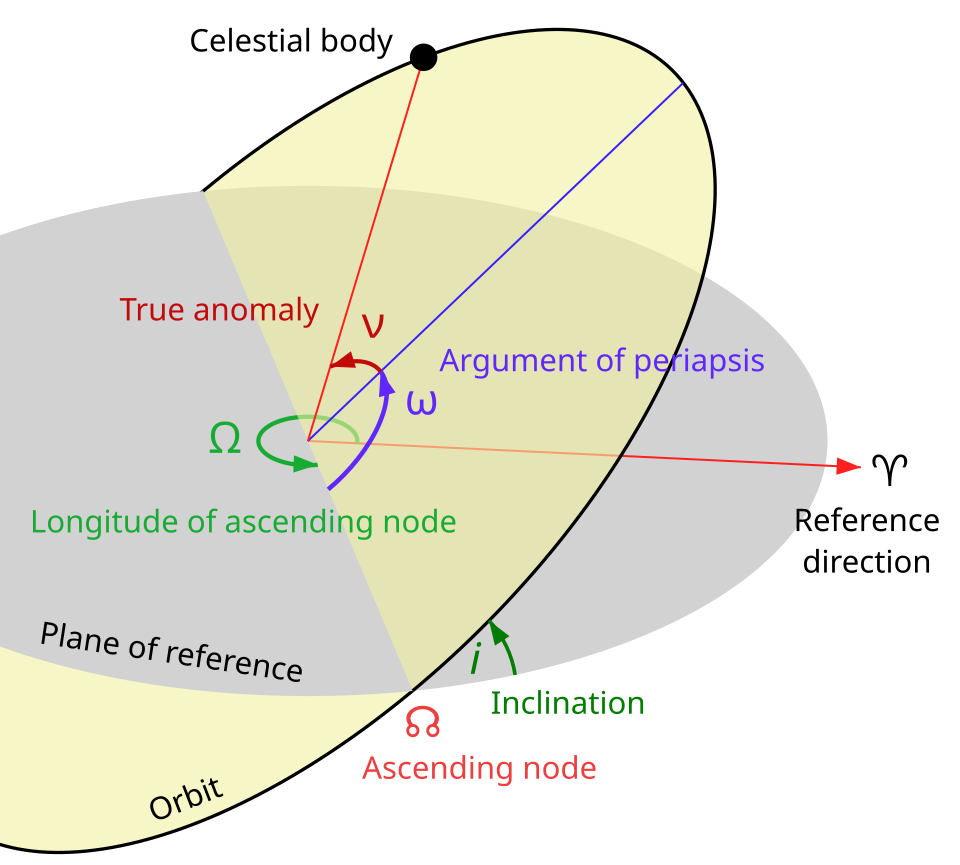
\includegraphics[scale=0.18]{images/ClassicalElements.png}
    \end{column}%
    \hfill%

    % Right Side
    \begin{column}{.48\textwidth}

      \begin{center}
      \begin{tabular}{c|c}

        Element & Function \\
        \hline\hline

        $i$ & \multirow{3}{*}{Orientation} \\
        $\Omega$ \\ 
        $\omega$ \\ \hline
        $e$ & \multirow{2}{*}{Shape} \\
        $a$   \\ \hline
        $\nu$ & \multirow{1}{*}{Position} \\
      \end{tabular}
      \end{center}
    \end{column}%
  \end{columns}
  \begin{center}
  \end{center}
\end{frame}


\begin{frame}{Kepler and Euler}

  \begin{center}
    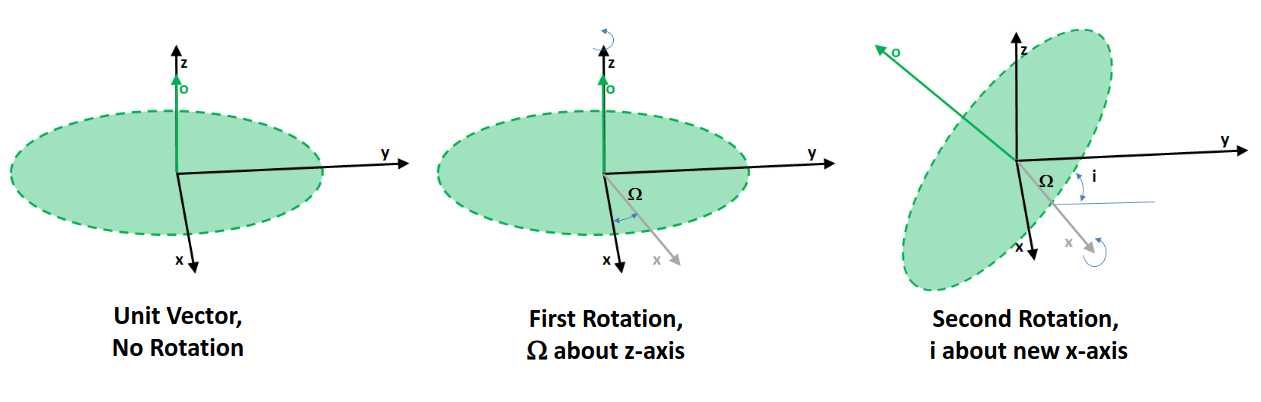
\includegraphics[scale=0.25]{images/OrbitAngles.png}
  \end{center}

  Kepler elements result in busy diagrams, but can be quite handy. E.g., $i$ and
  $\Omega$ directly define the direction of orbital momentum. 
  
\end{frame}


\subsection{Mean Element Theories}

\begin{frame}{Perturbation: Non-Sphericity}
  \[ \ddot{r} = \ddot{r}_\text{2B} + \ddot{r}_\text{PM} + \alert{\ddot{R}_\text{NS}} \]
  \begin{itemize}
  \item $\ddot{R}_\text{2B}$ uses point-mass equations
    \begin{itemize}
    \item Works for points
    \item Works for spheres (shell theorem)
    \end{itemize}
  \item Earth is neither
    \begin{itemize}
    \item Tidal forces (order meters)
    \item Centrifugal forces (order kilometers)
    \end{itemize}
  \end{itemize}
\end{frame}


\begin{frame}{Perturbation: Drag}
  \[ \ddot{R} = \ddot{R}_\text{2B} + \ddot{R}_\text{PM} + \ddot{R}_\text{NS}  + \ddot{R}_\text{IO} + \alert{\ddot{R}_\text{D}} \]

  \begin{itemize}
  \item Drag equation: $F_\text{D} = \frac{1}{2}\rho v^2 C_\text{D} A$
  \item Scales by
    \begin{itemize}
    \item Object shape and orientation ($C_\text{D}, A$).
    \item Square of object velocity $v^2$.
    \item Atmospheric density $\rho$, drops exponentially with altitude.
    \end{itemize}
  \item LEO objects (altitude $< 2000$ km) are low and fast
    \begin{itemize}
    \item experience non-negligible drag
    \end{itemize}
  \item Bonus: non-periodic and non-conservative.
  \end{itemize}
\end{frame}


\begin{frame}{Perturbation: et cetera}
  \[ \ddot{R} = \ddot{R}_\text{2B} + \ddot{R}_\text{PM} + \ddot{R}_\text{NS}  + \ddot{R}_\text{IO} + \alert{\ddot{R}_\text{D}} \]

  \begin{itemize}
  \item Drag equation: $F_\text{D} = \frac{1}{2}\rho v^2 C_\text{D} A$
  \item Scales by
    \begin{itemize}
    \item Object shape and orientation ($C_\text{D}, A$).
    \item Square of object velocity $v^2$.
    \item Atmospheric density $\rho$, drops exponentially with altitude.
    \end{itemize}
  \item LEO objects (altitude $< 2000$ km) are low and fast
    \begin{itemize}
    \item experience non-negligible drag
    \end{itemize}
  \item Bonus: non-periodic and non-conservative.
  \end{itemize}
\end{frame}

\begin{frame}{Osculating Elements}
  \[ \ddot{R} = \ddot{R}_\text{2B} + \ddot{R}_\text{PM} + \ddot{R}_\text{NS}  + \ddot{R}_\text{IO} + \ddot{R}_\text{D} + \alert{\ddot{R}_\text{SRP}}\]

  \begin{itemize}
  \item $\gamma := \sqrt{\frac{c^2}{c^2 - v^2}}$
  \item $ p = \gamma m v$
  \item photons: $m\rightarrow0, \gamma \rightarrow \infty $
    \begin{itemize}
    \item $p \rightarrow ?$
    \item God's math: $ p = \frac{h}{\lambda} $
    \end{itemize}
  \item Absorbing and emitting light imparts momentum
    \begin{itemize}
    \item Sunlight never stops: SRP
    \item Most impactful on higher altitude orbits
    \item Non-periodic and non-conservative
    \end{itemize}
  \end{itemize}
\end{frame}

\begin{frame}{Mean Elements}
  \[ \ddot{R} = \ddot{R}_\text{2B} + \ddot{R}_\text{PM} + \ddot{R}_\text{NS}  + \ddot{R}_\text{IO} + \ddot{R}_\text{D} + \alert{\ddot{R}_\text{SRP}}\]

  \begin{itemize}
  \item $\gamma := \sqrt{\frac{c^2}{c^2 - v^2}}$
  \item $ p = \gamma m v$
  \item photons: $m\rightarrow0, \gamma \rightarrow \infty $
    \begin{itemize}
    \item $p \rightarrow ?$
    \item God's math: $ p = \frac{h}{\lambda} $
    \end{itemize}
  \item Absorbing and emitting light imparts momentum
    \begin{itemize}
    \item Sunlight never stops: SRP
    \item Most impactful on higher altitude orbits
    \item Non-periodic and non-conservative
    \end{itemize}
  \end{itemize}
\end{frame}


\begin{frame}{SGP4 and TLEs}
  \[ \ddot{R} = \ddot{R}_\text{2B} + \ddot{R}_\text{PM} + \ddot{R}_\text{NS}  + \ddot{R}_\text{IO} + \ddot{R}_\text{D} + \alert{\ddot{R}_\text{SRP}}\]

  \begin{itemize}
  \item $\gamma := \sqrt{\frac{c^2}{c^2 - v^2}}$
  \item $ p = \gamma m v$
  \item photons: $m\rightarrow0, \gamma \rightarrow \infty $
    \begin{itemize}
    \item $p \rightarrow ?$
    \item God's math: $ p = \frac{h}{\lambda} $
    \end{itemize}
  \item Absorbing and emitting light imparts momentum
    \begin{itemize}
    \item Sunlight never stops: SRP
    \item Most impactful on higher altitude orbits
    \item Non-periodic and non-conservative
    \end{itemize}
  \end{itemize}
\end{frame}

\subsection{Limitations}

\begin{frame}{Inaccuracy I}
\end{frame}

\begin{frame}{Inaccuracy II}
\end{frame}

\begin{frame}{Imprecision}
\end{frame}

\section{TLE Differencing}
\subsection{General Approach}
\subsection{Subtleties}
\subsection{Experimental Verification}

\begin{frame}{TODO}
  TODO
\end{frame}

%% Q&A and Further reading.
\miniframesoff
\section*{}
\begin{frame}{References and Further Reading}
  \AtNextBibliography{\tiny}
  \nocite{*}
  \printbibliography
\end{frame}

\begin{frame}{Self Link}
  The source for this presentation is hosted at
\url{https://github.com/alan-christopher/edu/tle-differencing}.

\end{frame}
\end{document}
